\documentclass[11pt]{article}
%%%%%%%%%%%%%%%%%%%%%%%%%%%%%%%%%%%%%%%%%%%%%%%%%%%%%%%%%%%%%%%%%%%%%%%%%%%%%%%%%%%%%%%%%%%%%%%%%%%%%%%%%%%%%%%%%%%%%%%%%%%%%%%%%%%%%%%%%%%%%%%%%%%%%%%%%%%%%%%%%%%%%%%%%%%%%%%%%%%%%%%%%%%%%%%%%%%%%%%%%%%%%%%%%%%%%%%%%%%%%%%%%%%%%%%%%%%%%%%%%%%%%%%%%%%%
\usepackage{amsfonts}
\usepackage{eurosym}
\usepackage[spanish]{babel}
\usepackage[margin = 0.9in]{geometry}
\usepackage{amsmath,amsthm,amssymb}
\usepackage{graphicx}
\usepackage{comment}
%\usepackage[sort,comma]{natbib}
\usepackage[backend=biber, style = apa]{biblatex}
\usepackage{placeins} % to separate sections

\usepackage{adjustbox}
\usepackage{array}
\usepackage{multirow}
\usepackage{graphicx}
\usepackage{subcaption}
\usepackage{pifont}
\usepackage{amssymb}
\usepackage{comment}
\usepackage[utf8]{inputenc}
\usepackage{setspace}
\usepackage[hang, flushmargin, bottom]{footmisc}
\usepackage{footnotebackref}
\usepackage{xcolor}
\usepackage{hyperref}
\usepackage{booktabs}
\usepackage{pifont}
\usepackage{caption}
\usepackage{float}
\usepackage{todonotes}
\usepackage[normalem]{ulem} % for \sout{} strikethrough
\setcounter{MaxMatrixCols}{10}
%TCIDATA{OutputFilter=LATEX.DLL}
%TCIDATA{Version=5.50.0.2960}
%TCIDATA{<META NAME="SaveForMode" CONTENT="1">}
%TCIDATA{BibliographyScheme=BibTeX}
%TCIDATA{LastRevised=Sunday, April 28, 2024 18:12:38}
%TCIDATA{<META NAME="GraphicsSave" CONTENT="32">}
%TCIDATA{Language=American English}

%\setlength{\bibsep}{0.3pt}
\setlength{\textfloatsep}{5pt}
%\hypersetup{breaklinks=true,hypertexnames=false,colorlinks=true,citecolor = teal}
\captionsetup{font=normalsize}
\newcommand{\cmark}{\ding{51}}
\def\sym#1{\ifmmode^{#1}\else\(^{#1}\)\fi}
\renewcommand{\thetable}{\Roman{table}}
\geometry{verbose,tmargin=.9in,bmargin=1in,lmargin=1in,rmargin=1in,nomarginpar}
\makeatletter
\DeclareTextSymbolDefault{\textquotedbl}{T1}
\theoremstyle{plain}
\newtheorem{thm}{\protect\theoremname}
\theoremstyle{plain}
\newtheorem{prop}[thm]{\protect\propositionname}
\providecommand{\propositionname}{Proposition}
\providecommand{\theoremname}{Theorem}
\makeatother
\providecommand{\propositionname}{Proposition}
\providecommand{\theoremname}{Theorem}
\newtheorem{ass}[thm]{Assumption}
% \input{tcilatex}
\usepackage{tikz}
\usetikzlibrary{shapes.geometric, arrows, positioning}


\usepackage{titlesec}
% 2. Redefine the \section command to use a smaller font size
%    Here we use \large, which is one step smaller than the default \Large.
\titleformat{\section}
  {\normalfont\large\bfseries} % The format for the title (font, size, weight)
  {\thesection}               % The section number
  {1em}                       % The space between the number and title
  {}                          % Optional code before the title text



\addbibresource{../references.bib}
\begin{document}
\spacing{1.2}

 
\title{%{\Large Information sharing policies in financial services}\\
%o\\
{\Large Intercambio de Información y Competencia en Mercados Financieros}}
\author{
Diego Cussen\thanks{Estudiante de doctorado, New York University, \texttt{dc5004@nyu.edu}}
\quad \quad 
Lucas Schmitz\thanks{Estudiante de doctorado, Yale University,  \texttt{lucas.schmitz@yale.edu}}
} 
\date{\today}

\maketitle



\begin{center}
\fbox{\parbox{0.9\textwidth}{\color{red}\textbf{TODO --- Cosas por mejorar:}
\begin{itemize}
    \item Diferenciar nuestro trabajo de \textcite{foley_effects_2020}: ellos estudian un evento aislado (adquisición de un emisor no bancario por un banco) que afecta a un subconjunto del mercado. Nosotros estudiamos una reforma sistémica (REDEC) que incorpora a todos los OCNB simultáneamente, generando efectos de equilibrio general. Además, el REDEC fue anticipado, lo que requiere un enfoque estructural. Adicionalmente esto requiere un modelo estructural, pero para que queremos un modelo estructural? 
    \item Revisar si la pregunta de investigación necesita mayor especificidad.
    \item Pulir redacción general y acentos faltantes.
\end{itemize}
}}
\end{center}


\section{Plan de actividades}

\subsection{Propuesta: Motivación, datos y estrategia empírica}


% --- Version A (original) ---
%En mercados crediticios, la informacion permite a los bancos predecir el comportamiento de los consumidores. Por ejemplo, variables como un alto ingreso o un buen historial crediticio disminuyen la probabilidad de impago de un cliente. Una constante en este tipo de mercado es la asimetria de informacion entre bancos\footnote{En el mercado de crédito también existen asimetrías de información entre consumidores y bancos, las cuales generan selección adversa; véase, entre otros, \textcite{rothschild_equilibrium_1976}, \textcite{einav_selection_2011} y \textcite{einav_io_2021}. En este documento no nos enfocamos en seleccion adversa, sino que en asimetrías informacionales entre bancos.}. En particular, los bancos incumbentes conocen mejor a sus clientes que sus competidores.  Ademas del historial de pago, el banco incumbente observa variables como ingreso, ocupación y demanda por otros productos que el banco ofrece. Esta información adicional le permite estimar con mayor precisión el riesgo crediticio del cliente, y con ello obtener una ventaja informacional. Dicha ventaja informacional genera poder de mercado y distorsiones en la asignación del crédito.

% --- Version B (propuesta) ---
En mercados crediticios, la información permite a los acreedores evaluar el riesgo de sus clientes. Variables como el ingreso, la ocupación y el historial de pago ayudan a predecir la probabilidad de impago de un deudor. Un rasgo estructural de estos mercados es la asimetría de información entre acreedores\footnote{En el mercado de crédito también existen asimetrías de información entre consumidores y bancos, las cuales generan selección adversa; véase, entre otros, \textcite{rothschild_equilibrium_1976}, \textcite{einav_selection_2011} y \textcite{einav_io_2021}. En este documento no nos enfocamos en selección adversa, sino en asimetrías informacionales entre acreedores.}: el banco incumbente --- aquel con quien el cliente ya mantiene una relación --- observa no solo su historial de pago, sino también su ingreso, ocupación y demanda por otros productos financieros. Esta información le permite estimar con mayor precisión el riesgo crediticio del cliente, otorgándole una ventaja informacional respecto de sus competidores. Dicha ventaja genera poder de mercado para el incumbente y distorsiones en la asignación del crédito \parencite{sharpe_asymmetric_1990, dellariccia_information_2004}.


 
 

\begin{itemize}
    \item Medidas mitigatorias generales%: los gobiernos enfrentan la asimetría de información mediante sistemas de información crediticia. Introducir la ``nómina de deudores'' chilena (Art.\ 14 LGB) como sistema base: bancos, cooperativas y sociedades de apoyo al giro reportan y reciben información consolidada (archivo R04).
\end{itemize}
 
% --- Version B (propuesta) ---
Para mitigar estas asimetrías, los reguladores financieros establecen sistemas de información crediticia que obligan a los oferentes de crédito a compartir datos sobre sus deudores. En Chile, el principal instrumento ha sido la \textit{nómina de deudores}, establecida por el artículo 14 de la Ley General de Bancos (DFL~3 de 1997). Bajo este sistema, la CMF mantiene una base de datos consolidada (archivo R04) con la información de deuda reportada por las instituciones financieras fiscalizadas. El sistema opera bajo un principio de reciprocidad: las entidades que reportan a sus deudores son las mismas que reciben la información consolidada. Su objetivo es reducir la ventaja informacional del acreedor incumbente, permitiendo a sus competidores evaluar mejor el riesgo crediticio de potenciales clientes.

\begin{itemize}
    \item Historial cronológico de políticas chilenas%: (a) Leyes 20.455/20.522/20.575 (2010--2012) eliminan información de deudores del sistema; (b) Ley 21.130 (2019, implementada 2021--22) incorpora emisores de tarjetas no bancarios (ETNB); (c) Ley 21.680 REDEC (2024, vigente abril 2026) amplía a OCNB, compañías de seguro, cajas, securitizadoras, e incluye info positiva; (d) Ley Fintec (2023) establece banca abierta vía APIs.
\end{itemize}   

 
% --- Version B (propuesta) ---
En los últimos veinte años, el marco regulatorio chileno en materia de información crediticia ha experimentado múltiples reformas. Entre 2010 y 2012, tres leyes sucesivas (Leyes 20.455, 20.522 y 20.575) \textit{restringieron} la información disponible en el sistema. Estas leyes eliminaron registros de morosidad para desempleados de corto plazo, excluyeron consultas crediticias del puntaje, y borraron historiales de impago por montos menores a aproximadamente \$1.500 USD, afectando a 2,8 millones de personas \parencite{liberman_equilibrium_2018, madeira_impact_2024}. En dirección opuesta, reformas posteriores han \textit{ampliado} el sistema. La Ley 21.130 de modernización bancaria incorporó entre 2021 y 2022 a los emisores de tarjetas de crédito no bancarios (ETNB) como reportantes y receptores de la nómina de deudores. La Ley 21.680, que crea el Registro de Deuda Consolidada (REDEC) y entra en vigencia el 1 de abril de 2026, expande significativamente el universo de entidades participantes. Finalmente, la Ley Fintec (Ley 21.521) establece un sistema de finanzas abiertas que permitirá el intercambio de datos financieros entre instituciones mediante APIs estandarizadas.
\begin{itemize}
    \item Descripcion REDEC: %expande de $\sim$4 a $\sim$10+ tipos de entidades reportantes; incorpora información positiva (no solo morosidad); requiere consentimiento previo del deudor para consultas. La novedad clave: oferentes de crédito no bancarios (cajas de compensación, compañías de seguro, securitizadoras, asesores crediticios Fintec) entran al sistema por primera vez.
\end{itemize} 


El REDEC introduce dos cambios sustanciales respecto del sistema anterior. Primero, amplía el universo de entidades participantes. Bajo el artículo 14 LGB, solo las instituciones financieras fiscalizadas reportaban y recibían información consolidada. El REDEC extiende esta obligación a oferentes de crédito no bancarios (OCNB), incluyendo cajas de compensación y compañías de seguro, entre otros.\footnote{La lista completa de entidades reportantes se establece en el artículo 2, letra e) de la Ley 21.680. Además de cajas de compensación y compañías de seguro, incluye agentes administradores de mutuos hipotecarios endosables, sociedades securitizadoras, asesores crediticios regulados por la Ley Fintec, y acreedores no fiscalizados que superen ciertos umbrales de actividad.} Segundo, incorpora información positiva --- datos sobre el comportamiento de pago y las condiciones de los créditos vigentes --- y no solamente datos de morosidad. Esto es relevante porque la información positiva permite a los competidores del incumbente identificar a los buenos deudores, que es precisamente el canal a través del cual el intercambio de información intensifica la competencia.

\begin{itemize}
    \item Pregunta de investigación
\end{itemize}
Dado que el REDEC modifica sustancialmente la estructura informacional del mercado crediticio chileno, surge la pregunta natural sobre sus consecuencias. El presente proyecto busca responder: \textbf{¿cómo afecta el REDEC (Ley 21.680) el equilibrio en el mercado crediticio?} Con un especial énfasis en los efectos heterogéneos que puede tener en distintos grupos de la población, como puede ser la reducción al acceso al crédito de individuos sin historial previo en el sistema.

\begin{itemize}
    \item Fuerzas teóricas
\end{itemize}
La respuesta a esta pregunta no es obvia, pues la literatura teórica identifica fuerzas contrapuestas asociadas al intercambio de información crediticia. Cuando la información sobre la calidad de los deudores se vuelve pública, la ventaja informacional del incumbente se reduce. Esto intensifica la competencia y disminuye las tasas de interés para los deudores de bajo riesgo \parencite{sharpe_asymmetric_1990, petersen_effect_1995}.

Sin embargo, la pérdida de rentas informacionales puede reducir el acceso al crédito de clientes nuevos o sin historial. Sin intercambio de información, el acreedor que invierte en conocer a un cliente nuevo puede recuperar esa inversión en el futuro, cobrándole tasas superiores a las competitivas gracias a su ventaja informacional. Si esa ventaja desaparece, el retorno esperado de otorgar crédito a clientes desconocidos cae, y con ello el incentivo a hacerlo \parencite{petersen_effect_1995, dellariccia_information_2004}. La evidencia empírica es consistente con ambas fuerzas: \textcite{foley_effects_2020} documentan que compartir más información aumenta la competencia por buenos deudores pero puede perjudicar la inclusión financiera.

En el contexto específico del REDEC, estas fuerzas se manifiestan de la siguiente manera: los deudores de OCNB --- históricamente ``invisibles'' para los bancos --- se vuelven observables. Esto beneficia a los buenos deudores de OCNB, que ahora estarán expuestos a ofertas competitivas. Pero la reducción de las rentas informacionales de los OCNB puede disminuir sus incentivos para otorgar crédito a nuevos clientes. En la sección \ref{sec:modelo} presentamos un modelo que formaliza estas fuerzas.

\begin{itemize}
    \item Relevancia institucional
\end{itemize}
Esta investigación está directamente alineada con el mandato institucional de la CMF. El artículo 1 de la Ley 21.000 encarga a la Comisión ``velar por el correcto funcionamiento, desarrollo y estabilidad del mercado financiero, facilitando la participación de los agentes de mercado y promoviendo el cuidado de la fe pública''. Nuestro proyecto contribuye a este mandato en dos dimensiones. Primero, al estudiar si el REDEC intensifica la competencia y reduce las tasas para deudores de bajo riesgo, generamos evidencia directa sobre si la reforma cumple su objetivo de promover el \textit{desarrollo} del mercado financiero. Segundo, al evaluar si la reforma reduce el acceso al crédito de nuevos entrantes, informamos sobre potenciales riesgos para la \textit{inclusión financiera}.




%\begin{figure}[!ht]
%    \centering
%    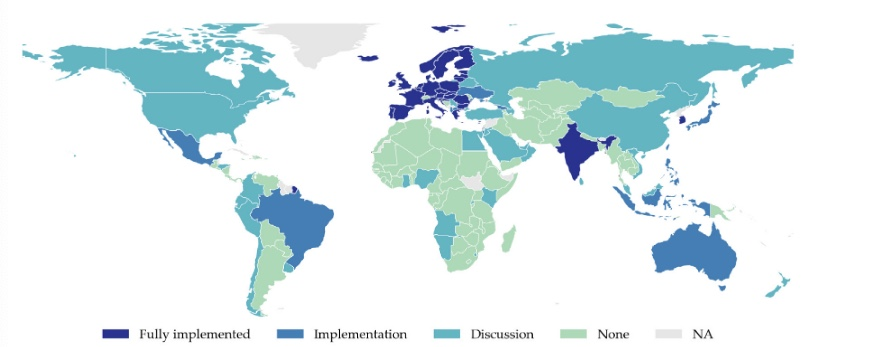
\includegraphics[width=0.8\linewidth]{../figures/Screenshots/map_babina2.jpeg}
%    \caption{Banca abierta en el mundo en 2021. \textit{Fuente}: \textcite{babina_customer_2025}.}
%    \label{fig:map_babina2}
%\end{figure}



 





En lo que sigue, detallaremos tanto los datos necesarios como los desafíos y enfoque empírico utilizado para responder a nuestra pregunta de investigación.

\newpage





 

\paragraph{Datos solicitados}


Para materializar esta investigación, 
los datos de alta frecuencia que requerimos de la Comisión para el Mercado Financiero (CMF) serían los siguientes:


\begin{itemize}
    \item Datos individuales de deudores sobre:
    \begin{itemize}
        \item Tarjetas de crédito bancarias y no bancarias: uso, pago y morosidad
        \item Préstamos individuales: montos, tasas de interés, planes de pago, vencimientos y morosidad
        \item Cuentas individuales (vista, corriente y de ahorro): saldos y movimientos
    \end{itemize}
\end{itemize}


Esta investigación está alineada con el mandato legal de la CMF, en particular, su rol de velar por la protección de los clientes y depositantes y promover el desarrollo del mercado financiero. 


 

\paragraph{Estrategia empirica}

Empiricamente nuestra investigación consta de dos partes. La primera parte presenta evidencia en forma reducida de los impactos de la ley REDEC. La segunda parte consiste en la estimacion de un modelo estructural del mercado del credito. 

Hay dos razones por las que la evidencia en forma reducida no es suficiente para estudiar el impacto de la reforma. Primero,  dado que los bancos anticipan la reforma, al estimar un modelo en forma reducida, podríamos encontrar un efecto nulo  de la reforma incuso en el caso de que si haya un efecto. A continuación presentamos nuestra estrategia empírica para obtener resultados en forma reducida. %% Aca deberiamos elaborar mas en los efectos anticipatorios, particularment podriamos usar v2 la parte de desafios empiricos para decir algo mas sobre el tema. 


La segunda razon es que un modelo estructural nos permite evaluar otros contrafactuales, como por ejemplo hacer una evaluacion prospectiva de las politicas de Finanzas Abiertas que seran implementadas este ano y tambien hacer una evaluacion de bienestar, que dado los efectos distributivos que se esperan de la reforma, es un aspecto relevante a estudiar. En la seccion \ref{sec:modelo} presentamos un modelo estructural simplificado que es la base sobre el cual se construira el modelo estructural completo que se estima usando los datos de la CMF.

A continuacion presentamos la estrategia empirica para obtener resultados en forma reducida.


El primer paso consiste en establecer una relación empírica entre la implementación de la ley REDEC y el acceso al crédito de los individuos con un perfil de crédito favorable. Para eso utilizamos un estudio de eventos\footnote{Para una introducción a los estudios de eventos ver \textcite{miller_introductory_2023}.},  que nos permite usar la variación en la entrada en vigor de la Ley REDEC para estimar sus efectos en el mercado financiero. Las dos especificaciones que estimamos son:
%El primer paso para identificar los efectos de la BA es establecer una relación empírica entre la implementación de la BA y la competencia en el mercado financiero y acceso a crédito en Chile. Para eso utilizamos un estudio de eventos\footnote{Para una introducción a los estudios de eventos ver \textcite{miller_introductory_2023}.},  que nos permite usar la variación en la entrada en vigor de la Ley Fintec para estimar sus efectos en el mercado financiero. La principal ecuación a estimar es:
\begin{equation}
    \Pr(y_{it}=y_{it}^P|y_{it} > 0, H_{it}= N) = f\left(
    \underbrace{\sum_{j\in \{-m,..., 0,...,n\}}\gamma_j D_{i,t-j}}_{\text{Estudio de eventos}} +
    \underbrace{\alpha_i
    %+ \delta_t
    }_{\text{Efectos fijos}} +
    \underbrace{\beta x_{it}}_{\text{Controles}} + e_{it}\right)
    \label{eqn:main_linear_model}
\end{equation}

\begin{equation}
    r_{it} =
    \underbrace{\sum_{j\in \{-m,..., 0,...,n\}}\gamma_j^r D_{i,t-j}}_{\text{Estudio de eventos}} +
    \underbrace{\alpha_i^r
    %+ \delta_t
    }_{\text{Efectos fijos}} +
    \underbrace{\beta^r x_{it}}_{\text{Controles}} + e_{it}^r
    \label{eqn:main_linear_model2}
\end{equation}

Las ecuaciones \ref{eqn:main_linear_model} y \ref{eqn:main_linear_model2} serán estimadas en la población de individuos con un buen historial crediticio. \footnote{Para clasificar a los individuos en términos de su historial crediticio podríamos usar técnicas de \textit{machine learning} siguiendo a \textcite{liberman_equilibrium_2018}. }
La ecuación \ref{eqn:main_linear_model} busca estimar el efecto de la BA en el tasa movilidad de clientes con un buen historial. La ecuación \ref{eqn:main_linear_model2} busca estimar el efecto de la BA en las tasas de interés a las cuales los clientes con buen historial se endeudan.

A continuación detallamos la notación usada. El sub-indice $i$ indexa individuos y $t$ indexa periodo de tiempo, por ejemplo mes. Los otros términos son:

\begin{itemize}
    \item $y_{it} \in \{0, 1, ..., N\}$ representa institución bancaria en la cual el individuo obtiene un crédito, donde $y_{it} = 0$ indica que el individuo no obtuvo un crédito en dicho periodo, e $y_{it} = b>0$ significa que obtuvo un crédito del banco indexado con el numeral $b$.
    \item $y_{it}^P$ representa el ultimo banco del cual el individuo obtuvo un crédito. Formalmente

    $$y_{it}^P =  \begin{cases}
        y_{it^-}\quad,  \text{si} \  t^- = \max\{s<t: y_{is}>0\} \ \text{existe} \\
        \emptyset \quad \quad , \text{si no hay historial previo}
    \end{cases}$$

    \item $H_{it}\in \{\emptyset, R, NR\}$ representa el historial crediticio del individuo. Donde $H_{it} =\emptyset$ indica que el individuo no tiene historial crediticio, $H_{it}= R$ indica que tiene un historial de impagos lo que implica que es un cliente riesgoso y $H_{it}= NR$ indica que en base a su historial es un cliente no riesgoso. Para clasificar a los individuos podríamos usar técnicas de \textit{machine learning} siguiendo \textcite{liberman_equilibrium_2018}.

    \item $D_{i, t-j}$ es una variable indicadora que toma el valor 1 si la politica de BA fue implementada $j$ periodos previo a $t$. Por lo que los coeficientes $\gamma_j$ capturan los efectos del tratamiento a lo largo del tiempo.

    \item $\alpha_i$ nos permiten capturar efectos individuales persistentes en el tiempo, por ejemplo que ciertos individuos tienen menores costos de búsqueda lo que genera un mayor \textit{switching rate}.

    \item $x_{it}$ son controles, que dependen de los datos a los cuales tengamos acceso, ellos permiten aislar efectos a nivel individual que son variables en el tiempo, por ejemplo el impacto de un aumento de los ingresos laborales del individuos o el impacto de la edad en el \textit{switching rate}.

    \item $f(x) = \exp(x)/(\exp(x) +1)$ es la función logística.
\end{itemize}


Los coeficientes de interés en la ecuación \ref{eqn:main_linear_model} son los $\gamma_j$ y en \ref{eqn:main_linear_model2} son los $\gamma_j^r$. Los coeficientes correspondientes a periodos posteriores a la implementación de la ley ($\gamma_j,  \gamma_j^r$ para $j \geq 0$) capturan los efectos de la BA, que pueden variar en el tiempo. La teoría previamente presentada predice que los $\gamma_j$ post-implementación sean positivos y que los $\gamma_j^r$ post-implementación sean negativos. Los coeficientes correspondientes a periodos previos a la implementación ($\gamma_j,  \gamma_j^r$ para $j < 0$) proveen un test placebo, por lo que esperaríamos que no fueran estadisticamente significativos.


%donde $y_{it}$ es una variable de resultado para un agente $i$ en periodo $t$, donde el periodo es relativo al mes en que la BA comenzó a afectar a ese agente. \textbf{explicar timing, controles, efectos fijos, residuo. tal vez buena idea explicar tendencias diferenciales, como caronine.}




Como se explicó antes, en presencia de efectos anticipativos no es posible estimar el impacto de la reforma en los clientes entrantes.
Por eso, el segundo paso es construir un modelo en que bancons compiten por otorgar créditos a clientes con distinta capacidad de pago. En un régimen sin BA, un banco con quien el cliente ya tiene una relación posee una ventaja informacional, pues es el único con datos detallados sobre la capacidad de pago del cliente. Con BA esta ventaja desaparece. Los bancos otorgan créditos repetidamente en el tiempo, sabiendo que la BA se implementará en el futuro. Usando los datos de la CMF antes, durante y después de la implementación de la ley Fintec, es posible estimar los parámetros que gobiernan el comportamiento de bancos y clientes. Estas estimaciones permiten estudiar en detalle los efectos de la BA incluso si los bancos anticipan la reforma, incluyendo sus efectos distributivos y sobre el bienestar de la población. Para fijar ideas, en el Anexo a este documento incluimos un modelo simplificado de este tipo.

% --- Version B (propuesta, adaptada a REDEC) ---
\paragraph{Estrategia empírica}

Empíricamente, nuestra investigación consta de dos partes. La primera presenta evidencia en forma reducida de los efectos del REDEC. La segunda consiste en un modelo económico estructural que permite interpretar los efectos de equilibrio y cuantificar el bienestar (ver sección \ref{sec:modelo}).

La evidencia en forma reducida no es suficiente por sí sola para evaluar el impacto completo del REDEC. Como se discutió en la sección anterior, los OCNB pueden anticipar la reforma y ajustar su comportamiento antes de la entrada en vigencia, lo que implica que estrategias basadas exclusivamente en la fecha de implementación podrían subestimar los efectos totales. A continuación presentamos las especificaciones en forma reducida.

La estrategia de identificación explota la variación de corte transversal generada por el REDEC. Antes de la reforma, los deudores que solo tenían créditos con OCNB eran invisibles para los bancos. Después del REDEC, su historial crediticio se vuelve observable. La muestra principal para las regresiones en forma reducida es el conjunto de individuos que tenían deuda exclusivamente con OCNB antes de la reforma. Dentro de esta muestra, definimos $Good_i = \mathbf{1}[\text{sin morosidad en OCNB}]$ como indicador de buen historial crediticio.\footnote{Para clasificar a los individuos podríamos usar técnicas de \textit{machine learning} siguiendo a \textcite{liberman_equilibrium_2018}.}

Estimamos tres especificaciones. La primera mide el efecto del REDEC sobre el acceso al crédito bancario:
\begin{equation}
    NuevoBanco_{it} = \beta^A \cdot (Post_t \times Good_i) + \gamma X_{it} + \delta_i + \theta_t + \varepsilon_{it}
    \label{eqn:access}
\end{equation}
donde $NuevoBanco_{it}$ es un indicador de si el individuo $i$ obtiene un crédito bancario en el período $t$, $Post_t$ indica los períodos posteriores a la entrada en vigencia del REDEC (abril 2026), $X_{it}$ son controles individuales variables en el tiempo, $\delta_i$ son efectos fijos individuales y $\theta_t$ son efectos fijos de tiempo. La teoría predice $\hat{\beta}^A > 0$: una vez que el historial de los deudores de OCNB se vuelve visible, los buenos deudores debieran recibir ofertas de bancos.

La segunda especificación mide el efecto sobre las tasas de interés:
\begin{equation}
    r_{ijt} = \beta^P \cdot (Post_t \times Good_i) + \gamma X_{it} + \mu_j + \theta_t + \varepsilon_{ijt}
    \label{eqn:pricing}
\end{equation}
donde $r_{ijt}$ es la tasa de interés del crédito otorgado al individuo $i$ por el acreedor $j$ en el período $t$, y $\mu_j$ son efectos fijos de acreedor. La teoría predice $\hat{\beta}^P < 0$: al poder distinguir entre buenos y malos deudores, los bancos ofrecen tasas más bajas a los buenos tipos en lugar de fijar una tasa única que los agrupe a todos (\textit{pooling}).

La tercera especificación mide el efecto sobre la calidad de los préstamos bancarios:
\begin{equation}
    Morosidad_{ijt} = \beta^D \cdot (Post_t \times DeudaOCNB_i) + \gamma X_{it} + \mu_j + \theta_t + \varepsilon_{ijt}
    \label{eqn:delinquency}
\end{equation}
donde $Morosidad_{ijt}$ indica si el individuo $i$ incurre en mora en un crédito otorgado por el banco $j$, y $DeudaOCNB_i$ indica si el individuo tenía deuda con OCNB antes de la reforma. Esta regresión se estima sobre el universo de créditos bancarios nuevos. La teoría predice $\hat{\beta}^D < 0$: al observar la deuda con OCNB, los bancos pueden filtrar a solicitantes con deuda oculta, mejorando la composición de su cartera.

En las tres especificaciones, los coeficientes pre-reforma proveen un test placebo: esperamos que no sean estadísticamente significativos para los períodos anteriores a abril de 2026.

Como se discutió previamente, la evidencia en forma reducida puede no capturar los efectos anticipatorios del REDEC sobre los clientes entrantes. Por eso, el segundo paso es estimar un modelo estructural en que acreedores compiten por otorgar créditos a clientes con distinta capacidad de pago. En el modelo, el acreedor incumbente posee una ventaja informacional sobre sus competidores, y el REDEC elimina (o reduce) dicha ventaja. Los acreedores otorgan créditos repetidamente en el tiempo, sabiendo que el REDEC se implementará en el futuro. Usando los datos de la CMF antes, durante y después de la implementación, es posible estimar los parámetros que gobiernan el comportamiento de acreedores y deudores. Estas estimaciones permiten cuantificar los efectos del REDEC incluso en presencia de anticipación, incluyendo sus efectos distributivos y sobre el bienestar. La sección \ref{sec:modelo} presenta un modelo simplificado que formaliza esta estructura.

 


%Como se explicó antes, en presencia de efectos anticipativos se espera que una ecuación como (\ref{eqn:main_linear_model}) sea incapaz de capturar completamente los efectos de la BA. Por eso, el segundo paso es construir un modelo en que bancons compiten por otorgar créditos a clientes con distinta capacidad de pago. En un régimen sin BA, un banco con quien el cliente ya tiene una relación posee una ventaja informacional, pues es el único con datos detallados sobre la capacidad de pago del cliente. Con BA esta ventaja desaparece. Los bancos otorgan créditos repetidamente en el tiempo, sabiendo que la BA se implementará en el futuro. Usando los datos de la CMF antes, durante y después de la implementación de la ley Fintec, es posible estimar los parámetros que gobiernan el comportamiento de bancos y clientes. Estas estimaciones permiten estudiar en detalle los efectos de la BA incluso si los bancos anticipan la reforma, incluyendo sus efectos distributivos y sobre el bienestar de la población. Para fijar ideas, en el apéndice a este documento incluimos un modelo simplificado de este tipo. 

\vspace{2cm} 


La primera contribución de este trabajo es un test empírico detallado de las teorías sobre los efectos de la información asimétrica en el mercado financiero. \textcite{sharpe_asymmetric_1990}, \textcite{petersen_effect_1995}, \textcite{dellariccia_adverse_1999} y \textcite{dellariccia_information_2004} notan que los efectos positivos de la competencia en el mercado financiero dependen de la extensión del problema de información asimétrica.

En el ámbito empírico, artículos relacionados son \textcite{petersen_benefits_1994,petersen_effect_1995}, \textcite{liberman_equilibrium_2018} y \textcite{foley_effects_2022}. El artículo más relacionado al presente trabajo es \textcite{foley_effects_2022}, que estudia la adquisición, en Chile, de un proveedor no bancario de tarjetas de crédito por parte de un banco. Esta adquisición fue una sorpresa, por lo que constituye un experimento natural. 

Al pasar a la cartera del banco, información sobre los clientes del prestamista no bancario (``el prestamista'') se volvió observable para otros bancos, aumentando la competencia por otorgar crédito a los clientes de ``buen tipo'' (alta acapcidad de repago) del prestamista. El costo es el riesgo de excluir a los prestatariosn más riesgosos, tal como predice la teoría. Crucialmente, los autores no encuentran que aumentar la información disponible resulte en mayor colusión -- un riesgo conocido en la literatura de organización industrial.\footnote{Papers de \textcite{green_noncooperative_1984}, Montag et al?, y Cussen and Montero (2024).}

Nuestro trabajo va significatimvemente más allá que \textcite{foley_effects_2022}. Primero, el cambio en el régimen informacional causado por la Ley Fintec afectará a todas las empresas y consumidores, creando efectos de equilibrio general que son difíciles o imposibles de capturar usando diferencia-en-diferencias. Por ejemplo, el experimento natural estudiado por \textcite{foley_effects_2022} solo aumenta la información de un subconjunto de empresas en el mercado (bancos) sobre una empresa de otro subconjunto (prestamistas no bancarios). La SFA haría pública toda la información, así que los bancos tendrían más información sobre los clientes de otros bancos, etc. ponerle color. 

Segundo, la Ley Fintec se aprobó años antes de su entrada en vigor. Luego, su efecto no puede medirse a partir del moemnto de su entrada en vigor, pues a ese momento los bancos ya habrán ajustado su comportamiento en cuanto a préstamos a nuevos clientes, y los clientes también pueden haber ajustado su probabilidad de repago, pues saben que serán observados por el resto del sistema financiero pronto.\footnote{Ver Pagano and Jappelli (1993), Padilla and Pagano (1997,200), citados en \textcite{foley_effects_2022}.} Las conisderaciones de este párrafo y el anterior llevan a concluir que una evaluación del efecto be implementar un SFA require un modelo estructural, como proponemos.

Finalmente, el uso de un modelo estrucutural nos permite medir los efectos distributivos y sobre el bienestar de un SFA y de políticas alternativas.

%\textcite{foley_effects_2020} estudian el efecto de la adquisición de un proveedor no bancario de tarjetas de crédito en Chile por parte de un banco. Al pasar a la cartera del banco, información sobre los clientes del prestamista no bancario se vuelve observable por otros bancos, lo que aumenta la competencia por otorgarles créditos. Los autores muestran que la competencia aumenta la eficiencia asignación de crédito entre clientes con capacidad de repago, a riesgo de excluir prestatarios más riesgosos del mercado. \textbf{EXPLICAR QUE EN FOLEY SOLO UNA EMPRESA CAMBIA DE REGIMEN, ENTOCNES NO PUEDE ESTIMAR EFECTOS DE EQUILIBRIO QUE SE DAN CUANDO TODAS LAS EMPRESAS CAMBIAN DE REGIMEN.} 

Tercero, este trabajo contribuye a una reciente literatura que estudia los impactos de la competencia en mercados con informacion asimetrica; ver \textcite{allen_search_2019}, \textcite{cuesta_price_2018} y \textcite{cosconati_competing_2025}. 



    \newpage
    \section*{Modelo de información asimétrica}
    \label{sec:modelo}
    {\small

    Este anexo resume el modelo  usado para formalizar cómo la asimetría informacional entre bancos y los costos de cambio (\textit{switching costs}) interactúan para determinar tasas de equilibrio, asignación de crédito e inclusión financiera.

    \paragraph{Juego en dos etapas (intuición)}
    \begin{enumerate}
        \item \textbf{Etapa 1 (producto introductorio).} Dos bancos compiten por captar al consumidor con un producto inicial (p.ej., cuenta corriente, tarjeta). Ex ante ninguno conoce el riesgo del consumidor.
        \item El banco elegido pasa a ser el \textbf{banco incumbente (\textit{home bank})} y observa información adicional durante la relación, aprendiendo el tipo $h$ del consumidor (probabilidad de default). El otro banco queda como \textbf{entrante no informado}.
        \item \textbf{Etapa 2 (mercado de crédito).} Ambos bancos compiten por otorgar un crédito. Si el consumidor se cambia al banco entrante, incurre un costo de cambio $\lambda\ge 0$.
    \end{enumerate}

    \paragraph{Etapa 2: demanda y utilidades}
    Una especificación estándar (logit) para la utilidad indirecta de endeudarse con el banco $j\in\{1,2\}$ es:
    \begin{align*}
        u_{1} &= -\alpha\, r_{1} + \varepsilon_{1}\\
        u_{2} &= -\alpha\, r_{2} - \lambda + \varepsilon_{2}
    \end{align*}
    donde $r_j$ es la tasa, $\alpha>0$ captura sensibilidad al precio y $(\varepsilon_1,\varepsilon_2)$ son shocks de preferencia. La probabilidad de elegir al incumbente es
    \begin{align*}
        s(r_1,r_2) = \frac{1}{1+\exp\!\big(\alpha(r_1-r_2)-\lambda\big)}.
    \end{align*}

    \paragraph{Etapa 2: costos, tipos y beneficios}
    El tipo $h\in(0,1)$ es la probabilidad de default. Con costo de fondeo normalizado a 1 por préstamo, la tasa de equilibrio de punto de quiebre para un tipo $h$ es $c(h)=\tfrac{1}{1-h}$. La ganancia esperada por préstamo (margen) es $(1-h)r-1$.

    El incumbente observa $h$ y puede fijar una tasa dependiente del tipo, $r_1=\sigma(h)$. El entrante no observa $h$ y fija una única tasa $r_2$.

    \paragraph{Etapa 2: caracterización de equilibrio (idea central)}
    En equilibrio, el banco informado fija (para cada tipo) una tasa igual a \textbf{break-even + markup}:
    \begin{align*}
        \sigma^*(h) = \frac{1}{1-h} + \underbrace{m_1\big(\sigma^*(h),r_2^*\big)}_{\text{markup}}.
    \end{align*}
    Bajo logit, el markup toma forma cerrada en función de la participación $s$:
    \begin{align*}
        \sigma^*(h) = \frac{1}{1-h} + \frac{1}{\alpha\big(1-s(\sigma^*(h),r_2^*)\big)}.
    \end{align*}
    El banco no informado elige $r_2^*$ maximizando su beneficio agregado (integrando sobre $h$), lo que genera una condición de primer orden que equivale a una regla de \textbf{break-even + markup promedio ponderado}. En el modelo, esto produce \textit{cream-skimming}: el incumbente retiene relativamente más a los tipos seguros y el entrante enfrenta una cartera adversamente seleccionada.

    \paragraph{Etapa 1: inducción hacia atrás y \textit{loss-leading}}
    La solución de etapa 2 determina el valor de ser incumbente (informado) versus entrante (no informado):
    \begin{align*}
        V^{I} &= \int \big[(1-h)\,\sigma^*(h)-1\big]\, s\big(\sigma^*(h),r_2^*\big)\, dF(h),\\
        V^{E} &= \int \big[(1-h)\,r_2^*-1\big]\, \big[1-s\big(\sigma^*(h),r_2^*\big)\big] \, dF(h),\\
        \Delta V &= V^{I}-V^{E}.
    \end{align*}
    Al competir en etapa 1 por captar al cliente, cada banco está dispuesto a sacrificar hasta $\Delta V$ en el precio del producto introductorio. Esto racionaliza \textbf{precios iniciales bajos (incluso bajo costo)} y, al mismo tiempo, \textbf{tasas más altas} en la etapa 2 por la interacción entre ventaja informacional y costos de cambio.

    }









\newpage
\printbibliography
 
\subsection{Graficos}
\end{document}